%-----------------------------------------------------------------------------
%
%               Template for sigplanconf LaTeX Class
%
% Name:         sigplanconf-template.tex
%
% Purpose:      A template for sigplanconf.cls, which is a LaTeX 2e class
%               file for SIGPLAN conference proceedings.
%
% Guide:        Refer to "Author's Guide to the ACM SIGPLAN Class,"
%               sigplanconf-guide.pdf
%
% Author:       Paul C. Anagnostopoulos
%               Windfall Software
%               978 371-2316
%               paul@windfall.com
%
% Created:      15 February 2005
%
%-----------------------------------------------------------------------------


\documentclass[preprint]{sigplanconf}

% The following \documentclass options may be useful:
%
% 10pt          To set in 10-point type instead of 9-point.
% 11pt          To set in 11-point type instead of 9-point.
% authoryear    To obtain author/year citation style instead of numeric.

\usepackage{amsmath}
\usepackage{graphicx}
\usepackage{subfig}
\usepackage{epstopdf}
\usepackage{fancyvrb}

\begin{document}

\conferenceinfo{PLDI '13}{16 June 2013 -- 21 June 2013, Seattle, Washington, USA.} 
\copyrightyear{2013} 
\copyrightdata{[to be supplied]} 

\titlebanner{banner above paper title}        % These are ignored unless
\preprintfooter{short description of paper}   % 'preprint' option specified.

\title{iMonitor: An Implicit-Signal Monitor}
\subtitle{}

\authorinfo{Wei-Lun Hung\and Vijay K. Garg}
           {The University of Texas at Austin}
           {wlhung@utexas.edu/garg@ece.utexas.edu}

\maketitle

\begin{abstract}
This is the text of the abstract.
\end{abstract}

\category{CR-number}{subcategory}{third-level}

\terms
term1, term2

\keywords
keyword1, keyword2

% code examples
\begin{SaveVerbatim}{ExplicitBoundedBuffer}
class BoundedBuffer {
  Object[] items;  
  lock mutex;
  condition notFull, notEmpty;
  int putPtr, takePtr, count;
  public void put(Object x) {
    mutex.lock();
    while(count == items.length) {
      notEmpty.signal();
      notFull.await();
    }
    items[putPtr++] = x;
    if(putPtr == items.length) {
      putPtr = 0;
    }
    ++count;
    notEmpty.signal();
    mutex.unlock();
  }
  public Object take() {
    mutex.lock();
    while(count == 0) {
      notFull.signal();
      notEmpty.await();
    }
    int x = items[takePtr];
    if(takePtr == items.length) {
      takePtr = 0;
    }
    --count;
    notFull.signal();
    mutex.unlock();
    return x;
  }
}
\end{SaveVerbatim}

\begin{SaveVerbatim}{iMonitorBoundedBuffer}
monitor class BoundedBuffer { 
  Object[] items; 
  int putPtr, takePtr, count; 
  public void put(Object x) { 
    waituntil(count < items.length); 
    items[putPtr++] = x; 
    if(putPtr == items.length) { 
      putPtr = 0; 
    } 
    ++count; 
  } 
  public Object take() { 
    waituntil(count > 0); 
    Object x = items[takePtr++]; 
    if(takePtr == items.length) { 
      takePtr = 0; 
    }
    --count;
    return x;
  }
}
\end{SaveVerbatim}

\begin{SaveVerbatim}{ImplicitNBoundedBuffer}
class BoundedBuffer {
  Object[] items;  
  lock mutex;
  condition noSufficientSpace;
  condition noSufficientItem;
  int putPtr, takePtr, count;
  public void put(int n) {
    mutex.lock();
    while(n + count > items.length) {
      noSufficientSpace.await();
    }
    for(int i = 0; i < n; ++i) {
      items[putPtr++] = new Object();
      if(putPtr == items.length) {
        putPtr = 0;
      }
    }
    count += n;
    noSufficientItem.signalAll();
    mutex.unlock();
  }
  public Object[] take(int n) {
    mutex.lock();
    while(count < n) {
      noSufficientItem.await();
    }
    Object[] ret = new Object[n];
    for(int i = 0; i < n; ++i) {
      ret[i] = items[takePtr++];
      if(takePtr == items.length) {
        takePtr = 0;
      }
    }
    count -= n;
    noSufficientSpace.signalAll();
    mutex.unlock();
    return ret;
  }
}
\end{SaveVerbatim}

\begin{SaveVerbatim}{iMonitorNBoundedBuffer}
monitor class BoundedBuffer { 
  Object[] items; 
  int putPtr, takePtr, count; 
  public void put(int n) { 
    waituntil(count + n <= items.length); 
    for(int i = 0; i < n; ++i) {
      items[putPtr++] = new Object(); 
      if(putPtr == items.length) { 
        putPtr = 0; 
      } 
    }
    count += n; 
  } 
  public Object[] take(int n) { 
    waituntil(count >= n);
    Object[] ret = new Object[n];
    for(int i = 0; i < n; ++i) {
      ret[i] = items[takePtr++]; 
      if(takePtr == items.length) { 
        takePtr = 0; 
      }
    }
    count -= n;
    return ret;
  }
}
\end{SaveVerbatim}
\begin{SaveVerbatim}{ExplicitRoundRobinMonitor}
public class RoundRobinMonitor{
  Lock mutex = new ReentrantLock();
  Condition[] conds;
  int numProc;
  int pid;
  public void access(int myId) {
    mutex.lock();
    while(pid != myId) {
      conds[pid].signal();
      conds[myId].await();
    }
    pid = (pid + 1) % numProc;
    conds[pid].signal();
    mutex.unlock();
  }
}
\end{SaveVerbatim}

\begin{SaveVerbatim}{iMonitorRoundRobinMonitor}
public monitor class RoundRobinMonitor {
  int numProc;
  int numAccess;
  public void access(int myId) {
    waituntil(pid == myId);
    pid = (pid + 1) % numProc;
  }
}
\end{SaveVerbatim}

\begin{SaveVerbatim}{ExplicitTicketReadersWriters}
public class ReadersWritersMonitor {
  int rcnt;
  int ticket, serving;
  Lock mutex;
  Map<Integer, Condition> mapCondition;
  public void startRead() {
    mutex.lock();
    int myTicket = ticket;
    ticket++;
    Condition cond = mutex.newCondition();
    mapCondition.put(myTicket, cond);
    while(myTicket != serving) {
      if(mapCondition.containsKey(serving)) {
         mapCondition.get(serving).signal();
      }
      cond.await();
    }
    mapCondition.remove(myTicket);
    rcnt++;
    serving++;
    mutex.unlock();
  }
  public void endRead() {
    mutex.lock();
    rcnt--;
    mutex.unlock();
  }
  public void startWrite() {
    mutex.lock();
    int myTicket = ticket;
    ticket++;
    Condition cond = mutex.newCondition();
    mapCondition.put(myTicket, cond);
    while(myTicket != serving || rcnt != 0) {
      if(myTicket != serving &&
           mapCondition.containsKey(serving)) {
         mapCondition.get(serving).signal();
      }
      cond.await();
    }
    mapCondition.remove(myTicket);
    mutex.unlock();
  }
  public void endWrite() {
    mutex.lock();
    serving++;
    mutex.unlock();
  }
}
\end{SaveVerbatim}

\begin{SaveVerbatim}{iMonitorTicketReadersWriters}
public monitor class ReadersWritersMonitor {
  int rcnt;
  int ticket, serving;
  public void startRead() {
    int myTicket = ticket;
    ticket++;
    waituntil(myTicket == serving);
    rcnt++;
    serving++;
  }
  public void endRead() {
    rcnt--;
  }
  public void startWrite() {
    int myTicket = ticket;
    ticket++; 
    waituntil(myTicket == serving && rcnt == 0);
  }
  public void endWrite() {
    serving++;
  }
}
\end{SaveVerbatim}

\section{Introduction} \label{sec:intro}
Developing efficient and robust concurrent programs within a limited time is 
critical than ever. On the one hand, the multi-core processor, which allows 
multiple threads to be executed at the same time, has become the mainstream of 
computers; however, the power of multi-core processors is limited due to the 
lack of concurrent applications. On the other hand, to compete with other rivals
and to satisfy consumer demands in software industry, an application needs to be
developed quickly. The concurrent programming is 
different from the traditional sequential programming. Multiple threads may 
interact with each other and try to access the same source. Therefore, providing
correctness of current programs is more difficult than sequential programs. In 
addition, the debugging process is panic in concurrent programs due to the 
thread scheduling. 

The monitor \cite{hoa74} is commonly used in concurrent programming for 
maintaining the mutual exclusion of shared resources and providing the 
synchronization mechanism between threads. Buhr and Harji \cite{bh05} divide 
monitors into two categories, the explicit-signal monitor and the 
implicit-signal monitor. Buhr and Harji use the explicit-signal monitor to 
simulate the implicit-signal monitor and point out that the implicit-signal 
monitor is not as efficient as the explicit-signal monitor. However, the 
implicit-signal is easy to be used and useful in concurrent programming,
especially for prototyping. 


Most programming languages, including the popular object-oriented language Java,
only provide the explicit-signal monitor but not implicit-signal. This research 
focuses on developing a framework supporting implicit-signal monitor without
sacrificing efficiency in the modern programming language - Java. 

our contribution

This paper is organized as follows. Section \ref{sec:pre} gives the
preliminaries. 
Our framework is presented in Section \ref{sec:fw} and the practical 
implementation details are discussed in Section \ref{sec:imp}. The proposed 
methods are then evaluated with experiments in Section \ref{sec:eval}. 
Section \ref{sec:conclu} gives the concluding remarks.
% You must have at least 2 lines in the paragraph with the drop letter
% (should never be an issue)

\section{Preliminaries} \label{sec:pre}
\subsection{Predicate}
A predicate which depends on some variables is a statement that is either true
or false. For example, $x > 0$ is a predicate where x is an integer variable. 
Predicates are commonly used to describe the properties of conditions. 
Predicates can be divided into two categories based on their variables.
\subsubsection{Global predicate} A predicate contains only shared variables of a
    monitor. 
\subsubsection{Local predicate} If both shared variables and local variables of a
    member function are in the predicate, which is called local predicate. 

\subsection{Monitor}
Monitor is an abstract object or module containing shared data to be used safely
by multiple member functions and threads in concurrent programming. Monitor can
be defined by two characteristics, mutual exclusion and synchronization. Mutual 
exclusion guarantees that at most one thread can execute any member function of 
a monitor at each time. The mutual exclusion provides programmers a more elegant
way to update shared data compared to directly accessing shared date. 
Synchronization maintains the executing order between threads. Threads may wait
for some condition to be met and release mutual exclusion temporarily. After the
condition has met, threads then re-acquire mutual exclusion and continue to 
execute.
According to Buhr and Harji \cite{bh05}, monitors can be divided into two 
categories based on the difference implementations of synchronization. 
  \subsubsection{Explicit-signal monitor} In this type of monitor, conditional
    variables
    and signal/await statement are used for synchronization. Programmers need to
    associate assertions with conditional variables manually. The mechanism of
    synchronization is achieved by two threads. One tread checks if some
    assertion is met or not and then explicit await if the assertion is not
    met. When another thread detects the state has changed and the assertion is
    met, and then explicitly signals appropriate threads in the monitor.
  \subsubsection{Implicit-signal monitor} This kind of monitor uses waituntil
    statements instead of conditional variables for
    synchronization. Programmers do not need to associate assertions with
    variables but use waituntil statements and logical predicate directly. In
    this kind of monitor, a thread will wait if the predicate of a waitutil
    statement is false, and execute the remaining tasks after the predicate
    has become true automatically.

Explicit-signal and implicit-signal monitors have different pros and cons. The 
explicit-signal has more complex syntax than the implicit-signal monitor. In 
addition, the explicit-signal needs the programmers to write the synchronization
mechanism manually, which increases the chance of writing incorrect code. 
However, in practice, explicit-signal is more efficient than implicit-signal. 
The implicit-signal monitor is still useful in prototyping and verification. 
Nevertheless, most of modern programming languages do not provide the 
implicit-signal monitor mechanism.




\subsection{Motivations for Implicit-Signal Monitor}
The concurrent programs are more difficult to be written and debugged than the 
sequential programs. Although explicit-signal monitor already provides an 
elegant mechanism for programmers to maintain mutual exclusion and synchronization 
in concurrent programs; implicit-signal is more straightforward in both code
reasoning and syntax. 

Fig.~\ref{fig:bb_exp} shows an example to
demonstrate the difference between implicit-signal monitor and explicit-signal 
monitor. The problem is producer-consumer problem, also known as bounded-buffer
problem. There are two kinds of threads, producers and consumers, which are 
trying to obtain access to the shared resources. Producers try to put items 
into the buffer and consumers try to take items out from the buffer. Every 
operation should be mutual exclusion. In addition, a producer cannot put any 
item when the buffer is full and a consumer cannot take any item when the 
buffer is empty. Fig.~\ref{subfig:bb_exam_exp} is written by the original Java
program language. A lock variable and conditional variables are
needed to maintain mutual exclusion and synchronization. A thread needs to
acquire the lock before entering member functions. In addition, programmers need
to explicitly associate the assertions with conditional variables and call
signal/await statement manually. Fig.~\ref{subfig:bb_exam_imp} shows a Java-alike
program for the producer-consumer problem. The key word $monitor$ for $class$
indicates that every member function of the class can only be executed at most
one thread at any time. In addition, the $waituntil$ statement indicates that if
the predicate of the waituntil is not true, the executing thread must wait and
release the monitor temporarily. After the predicate becomes true, the thread
then can awake automatically. As can be seen, Fig.~\ref{subfig:bb_exam_imp} is
more straightforward and simpler than Fig.~\ref{subfig:bb_exam_exp}. This research
focuses on developing a framework supporting such java-alike language without 
sacrificing efficiency.




\begin{figure}
  \centering
  \subfloat[Explicit-Signal] {
    \fbox{
      \BUseVerbatim[fontsize=\footnotesize]{ExplicitBoundedBuffer}
    }
    \label{subfig:bb_exam_exp}
  }
  \\
  \subfloat[Implicit-Signal] {
    \fbox{
      \BUseVerbatim[fontsize=\footnotesize]{iMonitorBoundedBuffer}
    }
    \label{subfig:bb_exam_imp}
  }
  \caption{Bounded-buffer example}
  \label{fig:bb_exp}
\end{figure}


\section{Framework of iMonitor} \label{sec:fw}
To make the implicit-signal available in the modern high-level language, Java, 
the iMonitor framework is proposed. Fig.~\ref{fig:framework} illustrates the 
framework of the iMonitor. The iMonitor takes a Java-extension program providing
the implicit-signal mechanism through supporting monitor class and waituntil 
statement. The iMonitor preprocessor transfers the iMonitor code into the 
tradition Java code which can be compiled with iMonitor library. The iMonitor 
Java library implements different kinds of implicit-signal monitor mechanisms. 
Programmers may choose one mechanism which is the most efficient for their 
requirements by providing some parameters to the preprocessor. Rewriting 
programs is unnecessary for different approaches of implicit-signal monitors. 
The flexibility is provided without any additional cost. 

\begin{figure}[ht!]
  \centering
  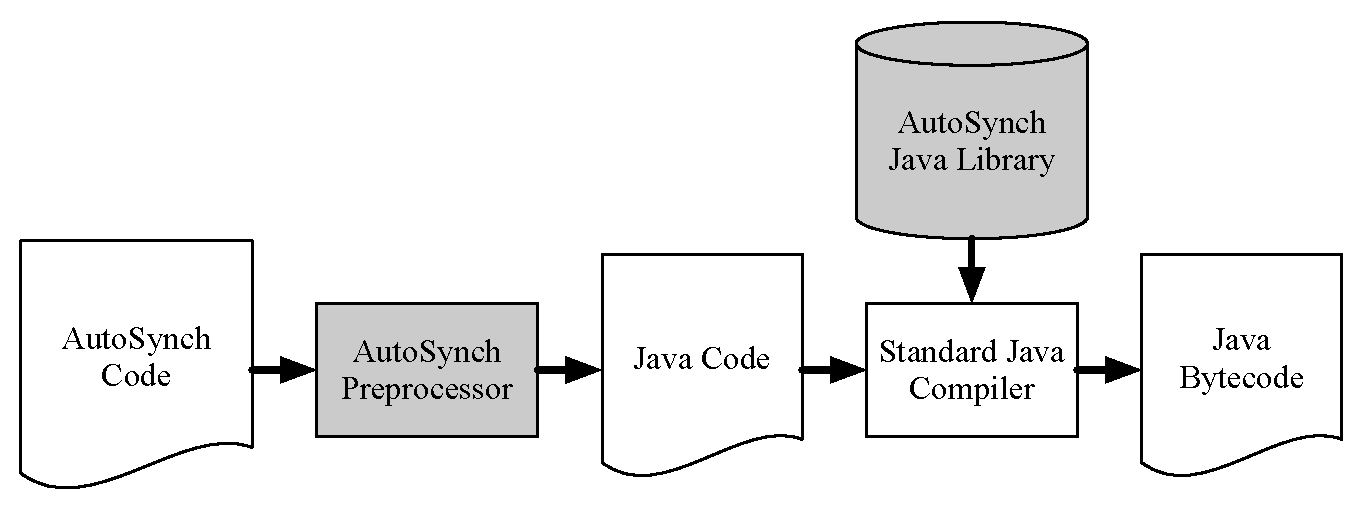
\includegraphics[width=80mm]{fig/flow.eps}
  \caption{The framework of iMonitor}
  \label{fig:framework}
\end{figure}

\section{Desirable Properties}
In this section, we discuss the properties which make the implicit-signal 
monitor available and efficient.

\subsection{Every thread can check predicates}
a distinguished thread v.s. a thread owns the monitor right to check the predicates.

\subsection{Less predicates need to be checked}
every time need to find a thread to run check less predicate 

\subsection{Reduce the number of content switch}
when signaling a thread, the thread continue to run

\section{Enabling Techniques}

\subsection{Globalization}
An operation called globalization is defined as replacing all local variables of
a predicate by its values at the time. The globalization converts a local 
predicate into a global predicate since all the local variables have been 
replaced. The globalization has an important characteristic that allows a
local predicate to be evaluated by any other thread safely after the original
thread waits. Since no other thread can access to local variables of a member 
function in which a particular thread is executing, values of local variables 
cannot be changed by other threads after the particular thread is waiting. 
Therefore, all other threads can check the globalized predicate safely. 


\subsection{Equivalence Predicate Reduction}

\subsection{Remove Local Predicate pairs as soon as possible}

\subsection{Only one executable thread is signaled}
reduce the number of content switch and the number of predicate checking 


\section{Practical Implementation} \label{sec:imp}

\begin{SaveVerbatim}{NaiveConstructorImp}

Lock L;
Condition C;
\end{SaveVerbatim}

\begin{SaveVerbatim}{NaiveEntryImp}

lock L 
\end{SaveVerbatim}

\begin{SaveVerbatim}{NaiveWaituntilImp}

if P is false
  signal all C
  do 
    wait C
  while P is false
\end{SaveVerbatim}

\begin{SaveVerbatim}{NaiveExitImp}

signal all C
unlock L
\end{SaveVerbatim}

\begin{SaveVerbatim}{NConditionConstructorImp}

Lock L
List<Predicate, Condition> LIST
foreach global predicate P
  create a pair <P, C>
  add <P, C> to LIST
\end{SaveVerbatim}


\begin{SaveVerbatim}{MapConditionConstructorImp}

Lock L
Map<Predicate, Condition> MAP
foreach global predicate P
  if P is not in MAP
    create a pair <P, C>
    add <P, C> to MAP 
\end{SaveVerbatim}

\begin{SaveVerbatim}{MapConditionWaituntilImp}

if P is a local predicate 
  PE := Globalization(P)
  if PE is not in MAP
    create a pair <PE, C>
    add <PE, C> to MAP
 
if P is false 
  foreach <PI, CI> in MAP
    if PI is true and CI has waiter
      signal CI
      break
  do 
    wait C
  while P is false

if P is local predicate 
    and C has no waiter
  remove <PE, C> from MAP
\end{SaveVerbatim}

\begin{SaveVerbatim}{MapConditionExitImp}

foreach <P, C> in MAP
  if P is true and C has waiter
    signal C
    break
unlock L
\end{SaveVerbatim}


The implementation of the implicit-signal monitor in iMonitor involves four 
parts:
\begin{enumerate}
  \item Monitor-constructor: the constructor of the monitor class, including 
    definitions and declarations of additional variables to provide mutual 
    exclusion and synchronization of monitor. 
  \item Monitor-function entry: executed before each member function, 
    involving declarations of additional variables and code to maintain
    mutual exclusion of monitor. 
  \item Monitor-waituntil statement: including declarations of additional
    variables and signal/await statements to implement the waituntil.
  \item Monitor-function leave: executed before the return statement of 
    each member function, involving code to guarantee mutual exclusion and 
    synchronization of monitor. 
\end{enumerate}


\subsection{Naive}

In the implementation of naive implicit-signal monitor, one lock variable, 
$L$, is declared for mutual exclusion, which should be acquired in 
the beginning of every member function and released before the return statement.
In addition, one conditional variable, $C$, is declared for 
synchronization, on which the implementation of waituntil depends. In the 
waituntil statement, the predicate expression is checked initially. If the 
expression is false; then all other threads which are waiting on $C$ are 
signaled to reevaluate their predicate expression since the monitor state may 
change. The current thread then is blocked in a loop and reevaluates its 
predicate expression when it is signaled. On the exit of a member function, 
all threads waiting on $C$ are signaled to reevaluate their predicate 
expression since the monitor state may change. Table \ref{tab:imp_naive} 
summarize the implementation of naive implicit-signal monitor. Although 
the naive implicit-signal monitor is easy to implement, it is inefficient. 
When a predicate is evaluated as false or a thread want to leave the monitor, 
all other threads waiting one the same monitor will be awaked and need to 
recheck their conditions.

\begin{table}
    \center
    \begin{tabular}{|l|l|} 
      \hline
      Constructor & \BUseVerbatim[baselinestretch=1.1]{NaiveConstructorImp}\\
      \hline
      Enter & \BUseVerbatim[baselinestretch=1.1]{NaiveEntryImp}\\
      \hline
      Waituntil $P$ & \BUseVerbatim[baselinestretch=1.1]{NaiveWaituntilImp}\\
      \hline
      Exit & \BUseVerbatim[baselinestretch=1.1]{NaiveExitImp} \\
      \hline
    \end{tabular}
    \caption{The naive implicit-signal monitor implementation}
    \label{tab:imp_naive}
\end{table}


\subsection{Map-Condition}
The map-condition predicate uses the data structure map to store pairs of 
predicate and conditional variables. A predicate and a corresponding conditional
variable are treated as key and value respectively. For every global predicate, 
a corresponding conditional variable is created and the pair of a predicate and a
conditional variable is added to the map in the constructor. For every local 
predicate, the globalization has been applied to the local 
predicate. Every local variable is replaced in the local predicate by its value
at this point. The globalization does not affect on the results of 
predicate evaluations since other threads cannot change the value of local 
variables but only global variables. After applying globalization to
the local predicate, a new predicate with only global variable is derived. 
If the predicate has not been added to the shared map, then the new 
predicated is added to the map with a corresponding conditional variable.
Otherwise, the corresponding conditional variable can be found by searching the
predicate in the map. Hence, the number of creating and removing conditional
variables has been reduced. 


\begin{table}
    \center
    \begin{tabular}{|l|l|} 
      \hline
      Constructor & \BUseVerbatim[baselinestretch=1.1]{MapConditionConstructorImp}\\
      \hline
      Enter & \BUseVerbatim[baselinestretch=1.1]{NaiveEntryImp}\\
      \hline
      Waituntil $P$ & \BUseVerbatim[baselinestretch=1.1]{MapConditionWaituntilImp}\\
      \hline
      Exit & \BUseVerbatim[baselinestretch=1.1]{MapConditionExitImp} \\
      \hline
    \end{tabular}
    \caption{The map-condition implicit-signal monitor implementation}
    \label{tab:imp_map_cond}
\end{table}

\section{Evaluations} \label{sec:eval}
%\subsection{Saturation}
Four kinds of experiments were performed to evaluate the performances of the
explicit-signal monitor with original Java and the implicit-signal monitor with
iMonitor framework. All of the experiments were conducted on a machine with 16 
Intel(R) Xeon(R) X5560 CPUs and 64 GBs memory. 


Fig.~\ref{fig:pc_eval} shows the results of producer-consumer problem. The
x-axis indicates the number of producers and consumers; the y-axis indicates the
runtime in seconds. Total 512000 $put$ and $take$ operations were executed by
all producers and consumers. As expected, the naive approach is much slower than
others. Both N-Condition and map approaches are slightly slower in most cases.
This phenomenon can be explained as follows. Observe explicit-signal and 
implicit-signal approaches for the producer-consumer problem is shown in 
Fig.~\ref{fig:bb_exp}. In the implicit-signal approaches, there are only two 
waituntil statements with global predicates, $count > 0$ and 
$count < items.length$. In the naive approach, producers and consumers are
signaled every time when a thread await or want to leave the monitor. Therefore,
if a consumer waits because $count = 0$, all other consumers are awaken and
check the predicate $count > 0$. Such kind of operations is redundant and lead
to the inefficiency of naive implementation. The map
implementations only need to check two global predicates in a waituntil
statement and the exit of monitor. Hence, the N-Condition and map implementation 
has the similar performance and only slightly slower than the explicit-signal
monitor approach. 
\begin{figure}[ht!]
  \centering
  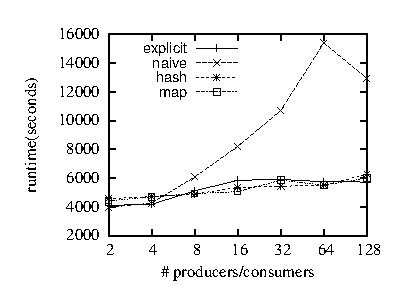
\includegraphics[width=80mm]{fig/pc.eps}
  \caption{The results of producer-consumer problem}
  \label{fig:pc_eval}
\end{figure}



\begin{figure}
  \centering
  \subfloat[Explicit-Signal] {
    \fbox{
      \BUseVerbatim[fontsize=\footnotesize]{ImplicitNBoundedBuffer}
    }
    \label{subfig:rbb_exam_exp}
  }
  \\
  \subfloat[Implicit-Signal] {
    \fbox{
      \BUseVerbatim[fontsize=\footnotesize]{iMonitorNBoundedBuffer}
    }
    \label{subfig:rbb_exam_imp}
  }
  \caption{Random Bounded-buffer example}
  \label{fig:rbb_exp}
\end{figure}
\begin{figure}[ht!]
  \centering
  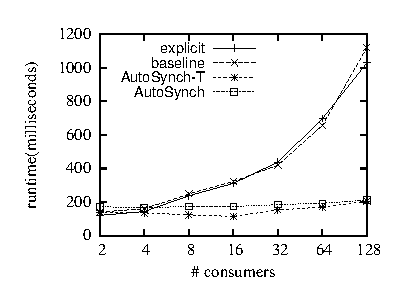
\includegraphics[width=80mm]{fig/rpc.eps}
  \caption{The results of random producer-consumer problem}
  \label{fig:rpc_eval}
\end{figure}

%Fig.~\ref{fig:rw_eval} shows the results of reader-writer problem. The
%x-axis indicates the number of readers and writers; the y-axis indicates the
%runtime in seconds. Total 1280 read/write operations were executed by all
%readers and writers. Since readers can read with each other at the same time.
%The runtime decreases as number of readers increases. Need to figure out why 
%explicit-signal approach is so slow in 1/5. Maybe the implementation? 
%
%\begin{figure}[ht!]
%  \centering
%  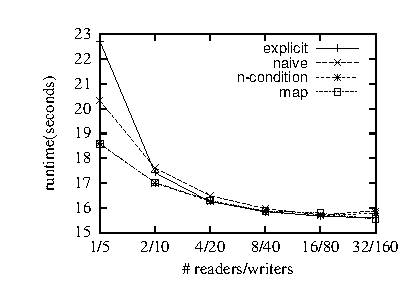
\includegraphics[width=80mm]{fig/rw.eps}
%  \caption{The results of reader-writer problem}
%  \label{fig:rw_eval}
%\end{figure}


%The dining philosophers problem is often used in computer science to describe 
%the synchronization issues. There are N philosophers siting around at a table 
%with a dish in front of them and a chopstick in between each philosopher. A 
%philosopher only think or eat. A philosopher needs to pick two chopsticks at the
%same time for eating and he does not put down a chopstick until he finishes 
%eating. If the chopstick is hold by another philosopher, then the philosopher 
%who want to eat must wait. In addition, a philosopher cannot eat forever, which
%means he will put down chopstick eventually. Every philosopher must be able to
%eat eventually if he is hungry. Figure 3. illustrate the experimental results
%of the dining philosophers problem. The x-axis depicts the runtime and the 
%y-axis describes the number of philosophers. As can be seen, three approaches 
%has the similar results. The implementations of Naive and N-condition are as 
%efficient as the implementation of explicit signal monitor. 
%
Fig.~\ref{fig:rr_eval} shows the results of round-robin access pattern. The
x-axis indicates the number of threads; the y-axis indicates the
runtime in seconds. In this set of experiments, threads are allowed to enter a
monitor in round-robin scheduling. Again, the results of N-Condition approach
are not shown because their performance is much worse than others. Total 
128000 operations were performed on the monitor. In this set
of experiment, the explicit-signal approach has an advantage since it can
explicitly to signal the next thread to enter the monitor. As can be seen, the
performance of explicit-signal approach is steady as the number of thread
increases. In comparison with our implicit-signal approaches, threads can only 
wait to enter the monitor. The runtime increases much as the number of thread 
increase in naive implementation. For the map approach, the performance is 
worse than the explicit-signal approach with a steady difference. 

\begin{figure}[ht!]
  \centering
  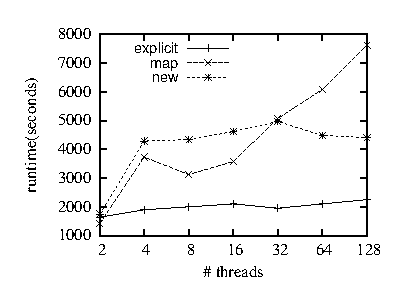
\includegraphics[width=80mm]{fig/rr.eps}
  \caption{The results of round-robin access pattern}
  \label{fig:rr_eval}
\end{figure}
\begin{figure}
  \centering
  \subfloat[Explicit-Signal] {
    \fbox{
      \BUseVerbatim[fontsize=\footnotesize]{ExplicitRoundRobinMonitor}
    }
    \label{subfig:rr_exam_exp}
  }
  \\
  \subfloat[Implicit-Signal] {
    \fbox{
      \BUseVerbatim[fontsize=\footnotesize]{iMonitorRoundRobinMonitor}
    }
    \label{subfig:rr_exam_imp}
  }
  \caption{Round-Robin example}
  \label{fig:rbb_exp}
\end{figure}

%\subsection{Practical}
%Fig.~\ref{fig:dp_eval} shows the results of dining philosophers problem. The
%x-axis indicates the number of philosophers; the y-axis indicates the
%runtime in seconds. Every philosopher performed 100 eat operations with a
%randomly thinking time between 1 to 20 
%milliseconds. Fig.~\ref{fig:dp_eval} does not show the results of N-Condition 
%implementations since the results are much worse than other implementations. It
%takes around 10 minutes for 128 philosophers. The reason is that many waituntil
%statements with local predicate are used in this problem. Therefore, many
%conditional variables are created and removed at runtime. As can be seen, the
%other three approaches have the similar results. This phenomenon can be
%explained as follows. The thinking time is much larger than the synchronization 
%time in the monitor. Therefore, the runtime is dominated by the thinking time.
%%These results suggest that if applications do not have many operations to access
%%a monitor, the performance will not have much difference in implicit-signal and
%%explicit-signal monitor.
%
%
%\begin{figure}[ht!]
%  \centering
%  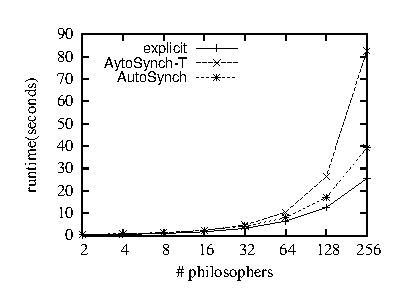
\includegraphics[width=80mm]{fig/dp.eps}
%  \caption{The results of dining philosophers problem}
%  \label{fig:dp_eval}
%\end{figure}


\begin{figure}
  \centering
  \subfloat[Explicit-Signal] {
    \fbox{
      \BUseVerbatim[fontsize=\footnotesize]{ExplicitTicketReadersWriters}
    }
    \label{subfig:rw_exam_exp}
  }
  \\
  \subfloat[Implicit-Signal] {
    \fbox{
      \BUseVerbatim[fontsize=\footnotesize]{iMonitorTicketReadersWriters}
    }
    \label{subfig:rw_exam_imp}
  }
  \caption{Random Bounded-buffer example}
  \label{fig:rbb_exp}
\end{figure}



\section{Conclusion} \label{sec:conclu}
The conclusion goes here. this is more of the conclusion



% use section* for acknowledgement
\section*{Acknowledgment}

The authors would like to thank...
more thanks here








\appendix
\section{Appendix Title}

This is the text of the appendix, if you need one.

\acks

Acknowledgments, if needed.

% We recommend abbrvnat bibliography style.

\bibliographystyle{abbrvnat}

% The bibliography should be embedded for final submission.

\begin{thebibliography}{}
\softraggedright

\bibitem {bh05}
  P. A. Buhr and A. S. Harji, \emph{Implicit-Signal Monitors}. ACM 
  Transactions on Programming Languages and Systems ACM, 27(6):1270-1343, 
  Nov. 2005.

\bibitem {hoa74}
  C. A. R. Hoare, \emph{Monitors: an operating system structuring concept}, 
  Commun.~ACM 17, 10(Oct. 1974), 549-557.



\end{thebibliography}

\end{document}
